%% Beamer Template of Sabine Hauert and R.~Eddie Wilson
%% Available on https://www.overleaf.com/latex/templates/eddies-minimum-beamer-style/qhcyjdqkbbgx#.V-vfg1SLS1I

%%%%%%%%%%%%%%%%%%%%%%%%%%%%%%%%%%%%%%%%%%%%%%
% Head matter - can we try to be consistent on
% included packages

\documentclass{beamer}
\mode<presentation>
{\usetheme{default}
 \usecolortheme{default}
 \usefonttheme{default}
 \setbeamertemplate{navigation symbols}{}
 \setbeamertemplate{caption}[numbered]} 

\usepackage[frenchb]{babel}
\usepackage[utf8x]{inputenc}
\usepackage{graphicx}
%\usepackage[frenchb]{babel}
\usepackage{amsfonts}
\usepackage{amsmath}
\usepackage{amssymb}
%\usepackage[T1]{fontenc}
\usepackage[utf8]{inputenc}
\usepackage{amsthm}
\usepackage{graphicx}
\usepackage{tikz}
\usepackage{tikz-cd}
\usepackage{hyperref}
\usepackage{amssymb}
\usepackage{geometry}

\hypersetup{                    % parametrage des hyperliens
    colorlinks=true,                % colorise les liens
    breaklinks=true,                % permet les retours à la ligne pour les liens trop longs
    urlcolor= blue,                 % couleur des hyperliens
    linkcolor= blue,                % couleur des liens internes aux documents (index, figures, tableaux, equations,...)
    citecolor= cyan               % couleur des liens vers les references bibliographiques
    }

\theoremstyle{definition}
\newtheorem{definition}{Definition}
\newtheorem{thm}{Theorem}
\newtheorem{ex}{Exercice}
\newtheorem{lem}{Lemma}
\newtheorem*{dem}{Proof}
\newtheorem{prop}{Proposition}
\newtheorem{cor}{Corollary}
\newtheorem{conj}{Conjecture}
\newtheorem{Res}{Result}
\newtheorem{Expl}{Example}
\newtheorem{rk}{Remark}

\newcommand{\N}{\mathbb N}
\newcommand{\Z}{\mathbb Z}
\newcommand{\R}{\mathbb R}
\newcommand{\C}{\mathbb C}
\newcommand{\Hil}{\mathcal H}
\newcommand{\Mn}{\mathcal M _n (\mathbb C)}
\newcommand{\K}{\mathbb K}
\newcommand{\B}{\mathbb B}
\newcommand{\Cat}{\mathbb B / \mathbb K}
\newcommand{\G}{\mathcal G }

\setlength\parindent{0pt}


\newcommand{\R}{\mathbb R}
\newcommand{\Z}{\mathbb Z}

\newtheorem{defn}{Definition}
\newtheorem{thm}{Théorème}

%%%%%%%%%%%%%%%%%%%%%%%%%%%%%%%%%%%%%%%%%%%%%%
% Formatting for title page
\title[First Steps with SCRATCH]{Expanseurs}
\author{Clément Dell'Aiera}
\institute{IECL}
\date{3 Octobre 2016}
%%%%%%%%%%%%%%%%%%%%%%%%%%%%%%%%%%%%%%%%%%%%%%

\begin{document}

\begin{frame}
  \titlepage
\begin{center}
\includegraphics[width=5cm]{IECL.png}\end{center}
\end{frame}

% PARTIE 1
\section{Un problème de théorie des réseaux}

\begin{frame}{Un problème de théorie des réseaux}
\begin{figure}
\href{run:InternetMap2012Full.avi}{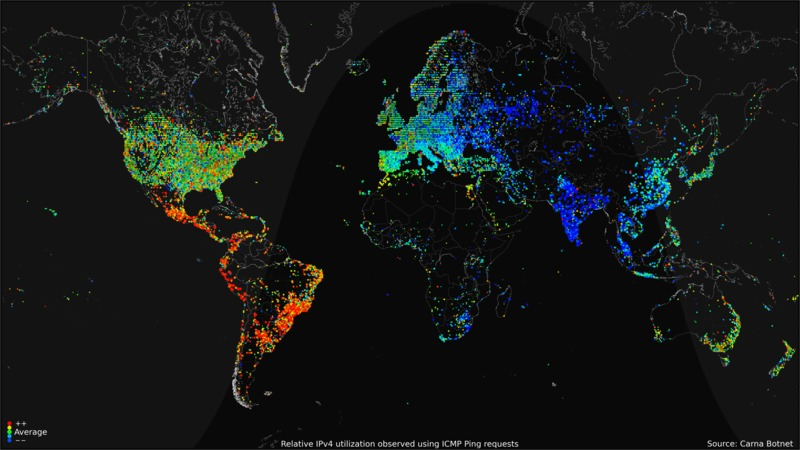
\includegraphics[scale=0.35]{InternetMap2012.jpg}} 
\caption{Map}
\end{figure}
\end{frame}

\begin{frame}{Un problème de théorie des réseaux}
Peut-on construire un réseau aussi grand que l'on souhaite sans que le risque de casse augmente tout en maîtrisant les coûts ?\\
Modélisation :\\
\begin{itemize}
\item[$\bullet$] Taille = nombre de sommets,
\item[$\bullet$] Propriété à maximiser = connexité,
\item[$\bullet$] Coûts = nombre d'arêtes.
\end{itemize}
Comment mesurer la connexité ? $\Rightarrow$ Marche aléatoire
\end{frame}

% PARTIE 2 
\section{Laplacien et marches aléatoires sur les graphes}

\begin{frame}{Laplacien}
Notations. Un graphe fini $G=(V,E)$.
 
\begin{itemize}
\item[$\bullet$] $V$ ensemble fini de $n$ sommets,
\item[$\bullet$] $E\subset V\times V$ l'ensemble des arêtes,
\item[$\bullet$] si $v\in V$, les voisins de $v$ : $N_v=\{w\in V / (v,w)\in E\}$,
\item[$\bullet$] le degré de $v$ : $deg(v)=|N_v|$.
\end{itemize}
Marche aléatoire uniforme sur un graphe :
\begin{enumerate}
\item $X_0=v_0$
\item $X_{n+1}|X_n\sim \mathcal U_{N_{X_n}}$. \\
\end{enumerate}
\end{frame}

\begin{frame}{Laplacien}
Le Laplacien sur un graphe $\Delta_G\in \mathcal L(l^2(X))$ est définit comme
\[(\Delta f) (x) = f(x) - \frac{1}{deg(x)}\sum_{y\in N_x} f(y) ,\]
si $f\in l^2(X)$.\\

Propriétés : $\Delta\geq 0$ et $\text{ker }\Delta\simeq \mathbb C $.\\

\[Sp(\Delta)= \lambda_0\leq \lambda_1\leq \lambda_2...\leq \lambda_n\]
et $\lambda_0=0$.
\end{frame}

\begin{frame}{Laplacien}

Si $M\in\mathcal L(l^2(X))$ est l'opérateur de Markov associé à la marche aléatoire, 
\[(Mf)(v)=\frac{1}{deg(v)}\sum_{w \in N_v} f(w) = \mathbb E[f(X_1)|X_0=v],\]
alors : \[\Delta=Id-M\]
Donc $0<\lambda_1$ contrôle la vitesse de convergence vers la distribution d'équilibre
\[\nu(x)= \frac{deg(x)}{\sum_{v\in V} deg(v)},\]
qui revient à tirer aléatoirement un somment avec une probabilité proportionelle à son nombre de voisin.
\end{frame}

\begin{frame}{Laplacien}
Reformulation du problème :\\
Peut-on construire une suite de graphes finis $\{X_j\}$ :
\begin{itemize}
\item[$\bullet$] de plus en plus grands $|X_j|\rightarrow \infty$,
\item[$\bullet$] $k$-réguliers : $deg(X_j)\leq k$,
\item[$\bullet$] uniformément connexes : $\exists\varepsilon>0, \forall j, \lambda_1(X_j)>\varepsilon$ 
\end{itemize}
\end{frame}

% PARTIE 3

\section{Expanseurs}

\begin{frame}{Expanseurs}
\begin{defn}
Un expanseur est une suite de graphes finis $\{X_j\}$ :
\begin{itemize}
\item[$\bullet$] de plus en plus grands $|X_j|\rightarrow \infty$,
\item[$\bullet$] $k$-réguliers : $deg(X_j)\leq k$,
\item[$\bullet$] uniformément connexes : $\exists\varepsilon>0, \forall j, \lambda_1(X_j)>\varepsilon$ 
\end{itemize}
\end{defn}
\end{frame}

\begin{frame}{Expanseurs}
\begin{figure}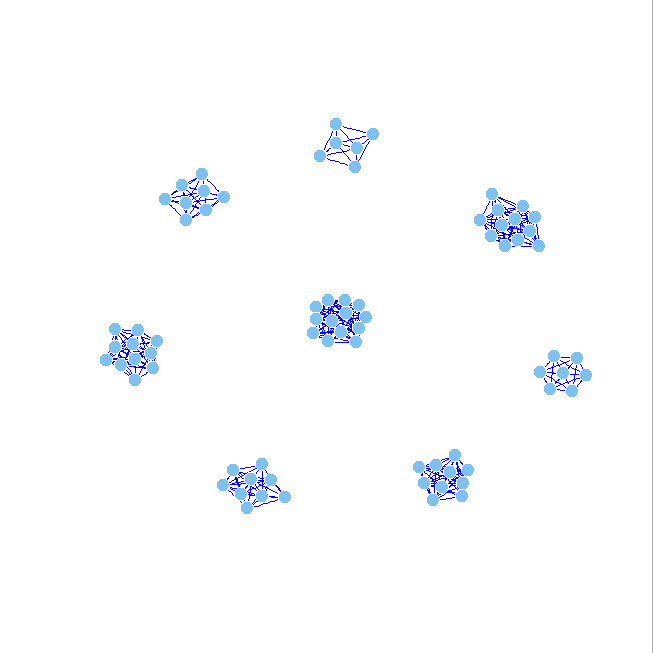
\includegraphics[scale=0.25]{Graphs5.png}\caption{Une famille de graphes}\end{figure}
\end{frame}

\begin{frame}{Expanseurs}
\begin{figure}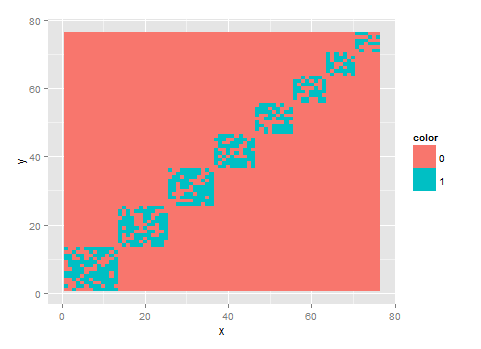
\includegraphics[scale=0.45]{Laplacian.png}\caption{Laplacien de la famille}\end{figure}
\end{frame}

\begin{frame}{Expanseurs}
Comment en construire ?
\end{frame}

\begin{frame}{Expanseurs} % Une motivation
Soit $\Gamma$ un groupe discret dénombrable finiement engendré, par une partie $S$ symmétrique telle que $e_\Gamma\not\in S $.\\
On construit un espace métrique $|\Gamma|$ grâce à la distance 
\[d_S(\gamma,\gamma')=l_S(\gamma^{-1}\gamma')\]
où $l_S$ est la longueurs des mots $l_S(g) = \min \{j \ |\ g=s_1 ...s_j \ , s_j\in S\}$.
Cette construction est canonique et ne dépend pas de $S$ !
\begin{thm}
Soient $S$ et $S'$ des parties finies génératrices. Alors les espaces métriques associés $(\Gamma,d)$ et $(\Gamma,d')$ sont quasi-isométriques.
\end{thm}
\end{frame}

\begin{frame}{Expanseurs}
\begin{figure}[h]\centering
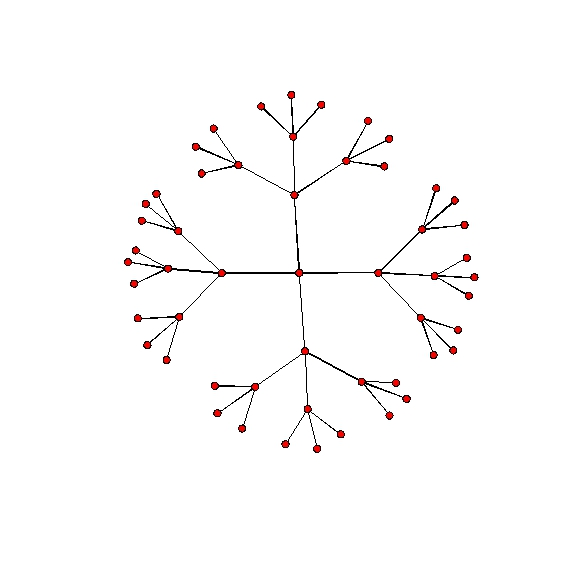
\includegraphics[scale=0.35]{CayleyFree2.jpeg}
\caption{Boules dans $Cay(\mathbb F_2)$}
\label{fig:Cayley}
\end{figure}
\end{frame}

\begin{frame}{Expanseurs}
\begin{figure}[h]\centering
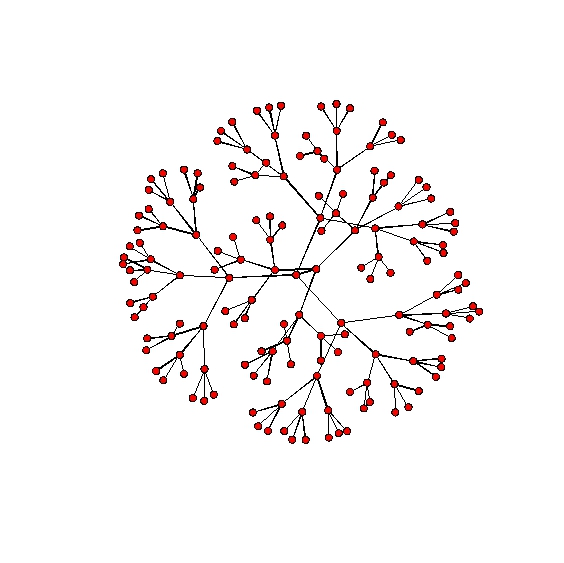
\includegraphics[scale=0.35]{CayleyFree3.jpeg}
\caption{Boules dans $Cay(\mathbb F_2)$}
\label{fig:Cayley2}
\end{figure}
\end{frame}
\begin{frame}{Expanseurs}
\begin{figure}[h]\centering
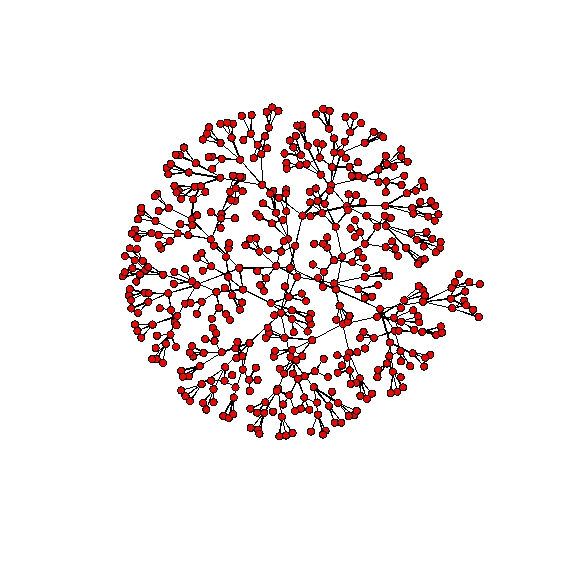
\includegraphics[scale=0.35]{CayleyFree4.jpeg}
\caption{Boules dans $Cay(\mathbb F_2)$}
\label{fig:Cayley3}
\end{figure}
\end{frame}
\begin{frame}{Expanseurs}
\begin{figure}[h]\centering
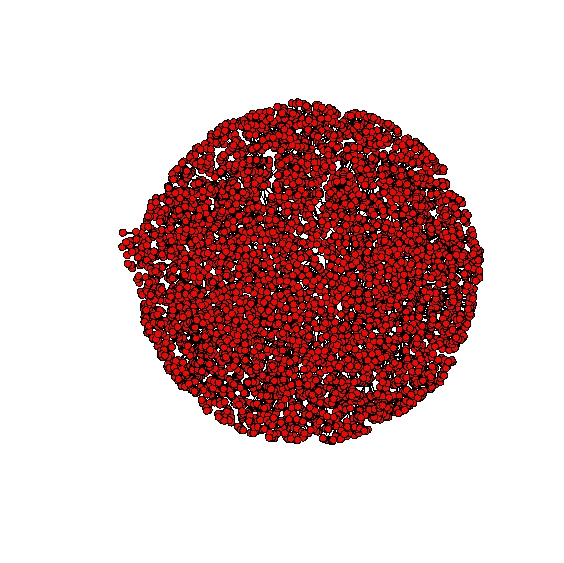
\includegraphics[scale=0.35]{CayleyFree5.jpeg}
\caption{Boules dans $Cay(\mathbb F_2)$}
\label{fig:Cayley4}
\end{figure}
\end{frame}

\begin{frame}{Expanseurs}
Recette pour fabriquer un expanseur.
\begin{itemize}
\item[$\bullet$] Choisir un groupe f.g. $\Gamma$, résiduellement fini par rapport à une famille de sous-groupes normaux $\Gamma_0 > \Gamma_1>...$ d'intersection triviale, et qui a la propriété T.
\item[$\bullet$] Former l'union dijointe (métrique...) des espaces $\Gamma/\Gamma_j$ :\[X_{\mathcal N}(\Gamma)=\sqcup_j \Gamma/\Gamma_j.\]
\item[$\bullet$] $X_{\mathcal N}(\Gamma)$ est un expanseur.
\end{itemize}

Exemple : $\Gamma = SL(3,\Z)$ et $ \Gamma_j = SL(3,p^j\Z)$.
\end{frame}

% PARTIE 4 
\section{Plongements uniformes}
\begin{frame}{Plongements uniformes}

\begin{defn}
Soit $X$ et $Y$ deux espaces métriques. Un plongement uniforme est une application $\phi : X\rightarrow Y$ telle qu'il existe deux applications croissantes $\rho_0,\rho_1 : \R_+^*\rightarrow \R_+^*$ vérifiant
\[\rho_0(d_X(x,y))\leq d_Y(\phi(x),\phi(y))\leq \rho_1(d_X(x,y))\] 
pour $x,y\in X$.
\end{defn}

\begin{itemize}
\item[$\bullet$] les isométries sont des plongements uniformes,
\item[$\bullet$] $\rho$ linéaires : les quasi-isométries,
\item[$\bullet$] $\Z\hookrightarrow \R$.
\end{itemize}
\end{frame}

\begin{frame}{Plongements uniformes} 
\begin{itemize}
\item[$\bullet$] Tout espace métrique se plonge isométriquement dans un espace de Banach.
\[\left\{\begin{array}{rcl} (X,d) &\rightarrow  & (l^\infty(X),d_\infty) \\ x &\mapsto  & d(x,-)- d(x_0,-)\end{array}\right.\]
\item[$\bullet$] Qu'en est-il des de plongement dans des espaces de Hibert ?
\end{itemize}
On se fixe $H$ un espace de Hilbert séparable.
\end{frame}

\begin{frame}{Plongements uniformes} 
\begin{thm}
Si ${X_j}_j$ est un expanseur, alors $X$ ne peut pas être plongé uniformément dans $H$.
\end{thm}
\end{frame}

\begin{frame}{Conséquences} 

La conjecture de Baum-Connes coarse donne un moyen de calculer les indices d'opérateurs elliptiques abstraits dans un espace métrique.\\
Elle est démontrée pour les espaces métriques qui admettent un plongement uniforme dans $H$, et admet des contre-exemples.\\
Une version modifiée de cette conjecture a été démontrée pour une classe d'expanseurs. \\
\end{frame}
%%%%%%%
%%%%%%%
%%%%%%%
%%%%%%%


\end{document}
